\documentclass[aspectratio=43]{beamer}
\usepackage[orientation=portrait, size=a0, scale=1.4]{beamerposter}
\setbeamersize{text margin left=1.5in,text margin right=1.5in} 
\usepackage[utf8]{inputenc}
\usepackage{graphicx}

\setlength{\parskip}{2.5\bigskipamount plus \smallskipamount minus \smallskipamount}
\setlength{\fboxrule}{2pt}
\setlength{\fboxsep}{2em}

\usepackage[numbers,square,sort]{natbib}
\usepackage{subcaption}
\newcommand{\sidebysidecaption}[4]{%
\RaggedRight%
  \begin{minipage}[t]{#1}
    \vspace*{0pt}
    #3
  \end{minipage}
  \hfill%
  \begin{minipage}[t]{#2}
    \vspace*{0pt}
    #4
\end{minipage}%
}
\setbeamertemplate{itemize items}[circle]

\usepackage{xcolor}

\definecolor{uiuc-blue}{HTML}{13294b}
\definecolor{light-gray}{HTML}{CFD5D8}
\usepackage{adjustbox}

\usepackage{multicol}
\usepackage{setspace}
\usepackage{ragged2e}
\usepackage{tabularx}

\usepackage{autonum}

\newcolumntype{Y}{>{\centering\arraybackslash}X}

\renewcommand{\baselinestretch}{1.0} 

\title{Phase-Based Video Motion Processing}
\author{Ruicheng Xian}

\begin{document}

\begin{frame}[t]

\setlength{\parskip}{0.5\baselineskip}

\makebox[\textwidth][c]{

\begin{adjustbox}{minipage=1.02\textwidth,margin=1.2in 0.3in 1.5in 1.1in,bgcolor=uiuc-blue,frame=0pt}

\newcolumntype{C}{>{\arraybackslash} m{0.8\textwidth} }\color{white}
\begin{tabular}{C m{0.2\textwidth}}
\huge \textbf{Phase-Based Video Motion Processing} 

\vspace{0.1em}

\normalsize Based on SIGGRAPH 2013 ``Phase based video motion processing'' paper by Wadhwa et al.

\vspace{1em}
\textbf{Sidan Qi, Huai Wu, Ruicheng Xian, Wanxian Yang}

\vspace{0.2em}

Department of Computer Science, University of Illinois Urbana--Champaign

& \begin{flushright} \includegraphics[scale=2.5]{uiuc.eps}\end{flushright}
\end{tabular}
\end{adjustbox}
}

\vspace{0.5em}

\begin{figure}[H]\centering
\makebox[\textwidth][c]{
\begin{adjustbox}{minipage=\linewidth,margin=0 0.1in,bgcolor=light-gray,frame=0pt}
\vspace{600px}
\caption{Results}
\end{adjustbox}}
\end{figure}



\vspace{0.5em}

\setlength{\columnsep}{0.8in}
\begin{multicols}{2}
\justify

\centerline{\large\textbf{Motivation and Overview}}

Many phenomena in real-life occurs at minuscule scales that are not perceptible with bare eyes, for instance, the swinging of skyscrapers due to winds, the pulsing change in skin color due to blood flow, or the wiggling of another person's eyes.  The goal of video motion processing is to magnify such barely noticeable motions that are present in recorded videos.

\textbf{Motion and Phase.} \ The motivation for phase-based video motion processing comes from the Fourier shift theorem.  A 1D image of unit length, denoted by $f\in\mathbb{R}^{[0,1]}$, can be written as a trigonometric polynomial using the definition of Fourier series.  With this representation, the shift theorem states that 
\begin{equation}
  f(x+\delta(t)) = \sum_{k=-\infty}^\infty c_k \exp\left(i2\pi k(x+\delta(t))\right),
\end{equation}
meaning that a translation on the image by distance $\delta(t)$ over time appears as a phase shift on the trigonometric polynomial.

By taking its phase component and use a temporal filter with zero DC response to extract the changing phase that corresponds to the translation, i.e. $\Delta\phi(t)=2\pi k \delta(t),$, we can directly magnify or attenuate this translation by increasing or decreasing the change in phase via multiplication, namely 
\begin{equation}
  f'(x+\delta(t)) = \sum_{k=-\infty}^\infty c_k \exp\left(i2\pi k(x+\delta(t))\right)\cdot \exp\left(i\alpha\Delta\phi(t)\right),
\end{equation}
for some magnification factor $\alpha$.

Usually, motions are localized such that we have to deal with $\delta(x,t)$, and they require multiple frequency bands to represent, meaning that by indexing the motions by $j$, we need to treat the phases over frequency bands $k\in A_j$ as a whole.  Then we write
\begin{equation}
  f(x+\delta(x,t)) = \sum_{j} \left(\sum_{k\in A_j} c_k \exp\left(i2\pi kx\right) \right) \cdot \exp
\left(i2\pi \sum_{k\in A_j}\delta_j(x,t,k)\right),
\end{equation}
and process each summand as a whose with temporal filters of appropriate pass-bands to isolate the motion of interest.


\textbf{Complex Steerable Pyramid.} \ Without further assumption, a simple method to partition the 2D frequency spectrum for motion extraction is the complex steerable pyramid.  Ideally, the complex pyramid divides the 2D frequency domain into the following regions.

Each partition captures objects of a certain size and orientation, hence motions of a certain scale and direction.  The aforementioned processing is performed on the signal contained in each partition.

\begin{figure}[tb]
\sidebysidecaption{0.48\columnwidth}{0.52\columnwidth}{%
  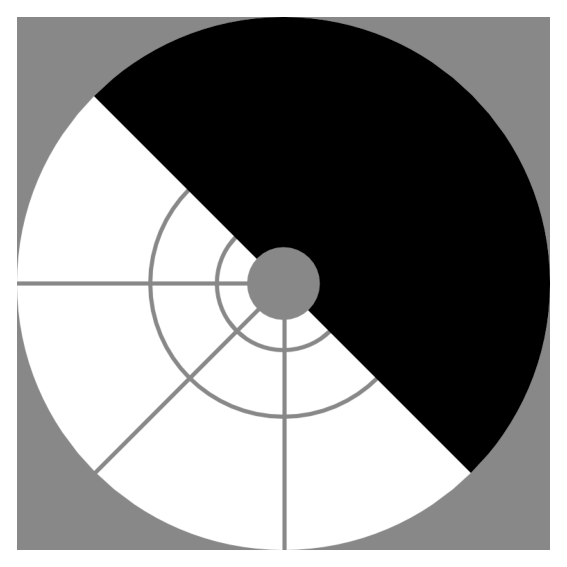
\includegraphics[scale=0.9]{pyramid.eps}~~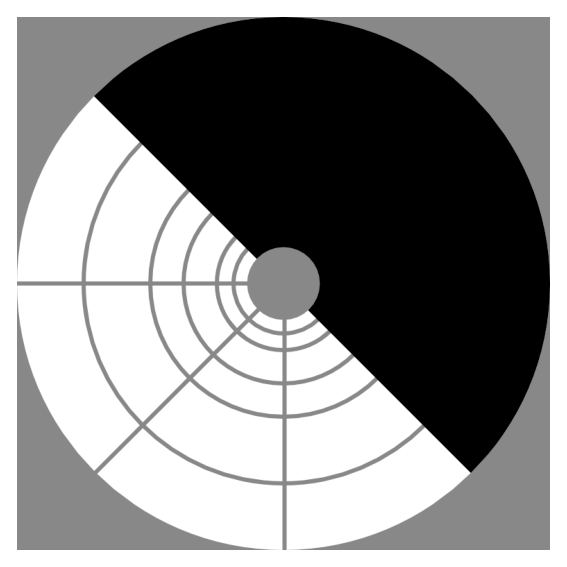
\includegraphics[scale=0.9]{pyramid-suboctave.eps}%
}{  \vspace{-0.3em}\caption{Ideal frequency response of the filters in a complex steerable pyramid of 3 levels and 4 orientations, meaning each of the 12 filters is an indicator function on a white partition. The right figure has suboctave bands.\\ \vspace{0.5em}
  The corners comprise the high-pass residual, and the center part is the low-pass residual. The black conjugate symmetric portion is discarded.
  }
}
\end{figure}

\vfill\break
\columnbreak

%\centerline{\large\textbf{Toy Example}}


\begin{figure}[tb]
\sidebysidecaption{0.61\columnwidth}{0.39\columnwidth}{%
\includegraphics[scale=1.6]{example.eps}%
}{%
\vspace{-0.3em}  \caption{In frame 2, the two boxes moved away from each other relative to frame 1.  The green curve is the result of motion magnification by 2 using difference of phase and a pyramid with 3 levels.
  }
}
\end{figure}



%\vspace{0.5em}
%\centerline{\large\textbf{Algorithm}}


\fbox{\begin{minipage}{0.95\columnwidth}
\textbf{Algorithm (Motion Modification).}

\vspace{0.5em}

\textbf{Input:}
\begin{itemize}
\item 
$I_{1:T}$ is a real-valued video sequence.
\item $D,K,N$ represents the depth, number of orientations and number of filters per octave of the complex steerable pyramid.
\item  $f_s$ represents the sampling rate of the video sequence, and $f_l,f_h$ represents the frequency range of the motion to be modified.
\item  $\alpha$ is the magnification factor.
\item  $B,F$ represent the types of filters to be used to construct the pyramid and for temporal filtering, respectively.
\end{itemize}

\vspace{0.3em}

\textbf{Initialize:}
\begin{itemize}
\item $P_{1:T}$, ${R_H}_{1:T}$, ${R_L}_{1:T}$ represent the pyramid sequence.
\item $Q_{1:T}$ represents the pyramid for storing motion magnified frames.
\item $J_{1:T}$ is the output video sequence.
\item Filter $F$ with $f_s,f_h,f_l$.
\end{itemize}

\begin{center}
  \noindent\rule{\textwidth}{2pt}
\end{center}

For $t=1,\cdots, T$, set $(P_t,{R_H}_t,{R_L}_t) \gets \text{PyramidAnalysis}(I_t,D,K,N,B)$, obtaining the complex steerable pyramid representation of each frame.
 
\vspace{0.3em}
 
For $d,n,k=1$ to $D,N,K$ respectively:
\begin{itemize}
\item Collect $X_{1:T} := (P_1[d,n,k],P_2[d,n,k],\cdots,P_T[d,n,k])$, the evolution of $I$ at scale $(D,N)$ and direction $K$.
\item Set $\Phi_{1:T}$ to be the phase component of $X_{1:T}$.
\item Set $\Delta\Phi_{1:T} \gets \text{TemporalFiltering}(\Phi_{1:T},F)$, which is to perform temporal filtering on the phase.
\item For $t=1,\cdots, T$, set $Q_t[d,n,k]\gets P_t[d,n,k] \circ \exp(i(\alpha-1)\Delta\Phi_t)$, which is to modify motion.
 \end{itemize}

For $t=1,\cdots, T$, set $J_t\gets \text{PyramidSynthesis}(Q_t,{R_H}_t,{R_L}_t,D,K,N,B)$, obtaining the motion magnified video sequence.

\vspace{0.3em}
Return $J_{1:T}$.
\end{minipage}}

\vspace{1em}
\centerline{\large\textbf{References}}

\nocite{*}
\bibliographystyle{plainnat}
\bibliography{refs}


\vfill\break
\end{multicols}
\end{frame}


\end{document}
